
\documentclass{article}
\usepackage[utf8]{inputenc}
\usepackage[T1]{fontenc}
\usepackage[frenchb]{babel}
\usepackage[bookmarks=true]{hyperref}
\usepackage{lmodern}
\usepackage{graphicx}


\author{Gentile Pierre, Didier-Roche François}
\date{\today}
\title{Document de spécification des exigences}

\frenchbsetup{StandardLists=true}
\begin{document}

\maketitle

\newpage
\tableofcontents
\newpage


\section{Introduction}
\subsection{Objet}
Appointime cherche à faciliter la prise de rendez-vous et l’accès aux disponnibilités des artisants/entreprises de services.
Elle permet de mettre en relation des particuliers et des artisants/entreprises de services intuitivement et rapidement.
\subsection{Portée du projet}
Appointime permet la mise en relation et la prise de rendez vous rapide pour des taches simples/de routine entre une entreprise et un client.
L’application sera donc divisée en deux: la partie particulier et la partie professionnelle.
\begin{itemize}
\item Le professionnel pourra indiquer ses disponibilités et précisera son domaine de compétances ainsi que les tâches de base qu’il peut éffectuer.
\item Le client quant à lui pourra faire des recherches selon ses
  besoins et trouver rapidement et intuitvement des professionnels
  disponibles aux alentours.
\end{itemize}
\subsection{Définitions, acronymes, abréviations}
\begin{itemize}
\item \textbf{Professionnel} : Ce terme décrit toutes les personnes ayant une entreprise proposant des
  services sur prise de rendez-vous.
\item \textbf{Pariculier} : Ce terme décrit toutes les personnes
  voulant prendre rendez-vous auprès d'un professionnel.
\item \textbf{Flashcode} : Un flashcode est un identifiant sous forme
  d'image en 2 dimension pouvant être lue par l'appareil photo d'un smartphone et
  interpreté par un programme.

\end{itemize}


\subsection{Références}

\subsection{Vue d'ensemble}


\section{Description générale}
\subsection{Environnement}
\begin{itemize}
\item Le système décrit est une application mobile sur IOS et
Android.
\item Le système est adapté pour n'importe quel smartphone ayant IOS ou Android comme
système d'exploitation.
\item Les actions de l'utilisateur s'éffectuent via l'écran
  tactile, le capteur d'empreintes digitales ou l'appareil photo du smartphone.
\item L'application communique avec une base de donnée distante
  via une connexion \og réseau mobile\fg{} ou Wifi.


%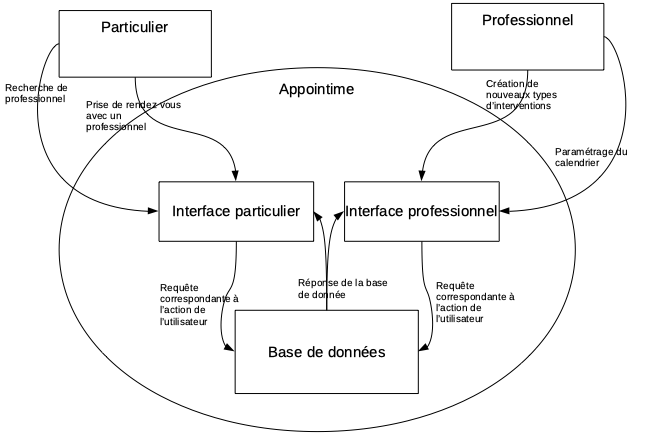
\includegraphics[scale=0.5]{ShematDiagrammes/ShematGeneral.png}
\end{itemize}
\subsection{Fonctions}
\begin{itemize}
\item L'application permet à n'importe quel professionnel de créer un
calendrier de rendez-vous personnalisé.
\item L'application permet à n'importe quel particulier de rechercher
  un professionnel.
\item L'application permet à n'importe quel particulier de prendre un
  rendez-vous chez un professionnel selon le calendrier paramétré par
  ce dernier.
\end{itemize}
\subsection{Caractéristiques des utilisateurs}
\begin{itemize}
\item L'utilisateur peut être soit un professionnel proposant des
  services sur prise de rendez-vous soit
  un particulier souhaitant rechercher un professionnel et prendre un
  rendez-vous avec ce dernier.
\item Les utilisateurs n'ont besoin d'aucune connaissances techniques.
\end{itemize}
\subsection{Contraintes}
\begin{itemize}
\item La prise et l'annulation de rendez-vous doit se plier à la
  politique de chaque professionnel.
\item Les informations des utilisateurs devront uniquement être
  utilisées dans le cadre de l'application.
\end{itemize}
\subsection{Hypothèses et dépendances}
\subsubsection{Systeme d'exploitation}
\paragraph{Systeme d'exploitation Apple}
Nous supposons que l'application sera utilisée sur une version d'IOS superieure ou egale à IOS 8.
\paragraph{Systeme d'exploitation Android}
Nous supposons que l'application sera utilisée sur une version d'Android superieure ou égale à Android 5.0.
\paragraph{Acces au réseau}
Nous supposons que les appareils utilisant l'application seront reliés à internet.

\section{Exigences spécifiques}
\subsection{Exigences des interfaces externes}
\subsubsection{Interfaces avec les utilisateur}
\paragraph{Les informations des utilisateurs :}
\begin{itemize}
 \item Un formulaire d'inscription doit permettre à l'utilisateur de
   s'inscrire en entrant différents champs textuels (email,
   confirmation de l'email, mot de
   passe, confirmation du mot de passe, nom d'utilisateur, numéro de téléphone, adresse) nécéssaires au
   système , ainsi qe de cocher : \og Professionnel? \fg{} et en appuyant sur
   un bouton \og S'inscrire \fg{}.

%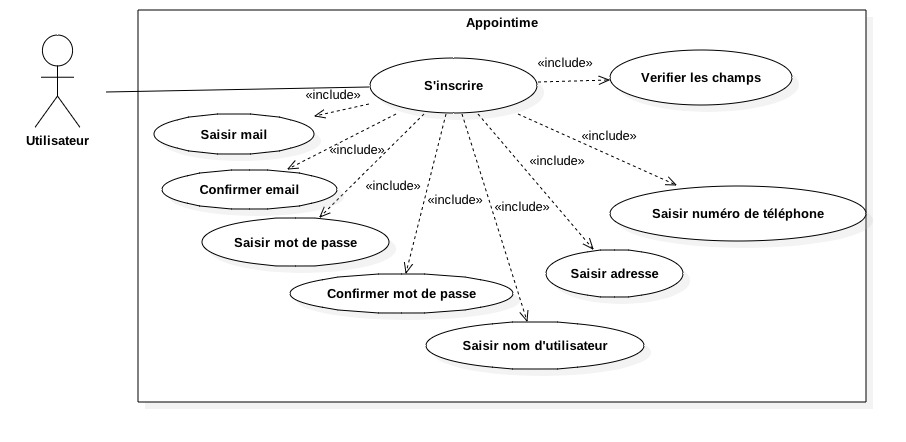
\includegraphics[scale=0.5]{ShematDiagrammes/useCaseInscription.jpg}
\item Si l'utilisateur est un professionnel, un formulaire doit lui permettre de renseigner les informations relatives 
à son entreprise (nom,description du type de services, description générale, numéro de siret)

\item Si l'utilisateur est un professionnel, un formulaire doit lui permettre de renseigner les informations relatives aux 
horaires d'ouverture de son entreprise (heure d'ouverture et fermeture pour chaque demie journée de la semaine)

\item Un formulaire doit permettre à un utilisateur de modifier les
  informations mentionnées durant son inscription.
\item Un formulaire de connexion doit permetre à un utilisateur de
  s'identifier pour avoir accès aux services du système en entrant
  différents champs textuels (email, mot de passe) et en appuyant sur
  un bouton \og Se connecter \fg{}.

%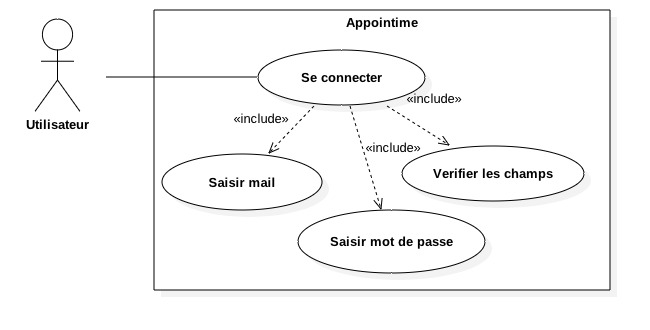
\includegraphics[scale=0.5]{ShematDiagrammes/useCaseConnexion.jpg}

\item Une reconnaissace par empreinte digitale devrait permette à un
  utilisateur de pouvoir s'identifier rapidement dans le cas ou cette
  fonctionnalitée est diponible sur le téléphone.
\item Une reconnaissance faciale devrait permette à un
  utilisateur de pouvoir s'identifier rapidement dans le cas ou cette
  fonctionnalitée est diponible sur le téléphone.
\end{itemize}
\paragraph{Préférences des utilisateurs :}
\begin{itemize}
\item Le client doit pouvoir acceder à la page \og Paramètres \fg{} de l'application en
  appuyant sur un bouton \og Menu \fg{} puis \og Préférences \fg{}
  dans la liste déroulante qui viens de s'afficher à l'écran.
\item Le client doit pouvoir activer ou désactiver les notifications
  de l'application dans le menu paramètres.
\item Le client devrait pouvoir modifier le son des notification
  (volume et tonalitée) dans la page paramètres.
\item Le client devrait pouvoir activer le thème nuit, qui modifierait les
  couleurs de l'application, dans la page paramètres.
\end{itemize}
\paragraph{Recherche d'un professionnel :}
\begin{itemize}
\item Un champs textuel doit permettre à l'utilisateur d'éffectuer une
  recherche par profession, par nom
  d'entreprise ou via un flashcode fournit par le professionnel. Dans
  les deux premiers cas, l'utilisateur devrait pouvoir selectionner
  un périmetre maximal de recherche si il le souhaite.
\item Après avoir fais une recherche, le client doit pouvoir sélectionner un
  professionnel dans la liste affichée.
\item Le particulier doit pouvoir ajouter un professionnel en favoris grâce
  à un bouton présent sur le calendrier d'un professionnel et sur la
  liste déroulante de recherche.

%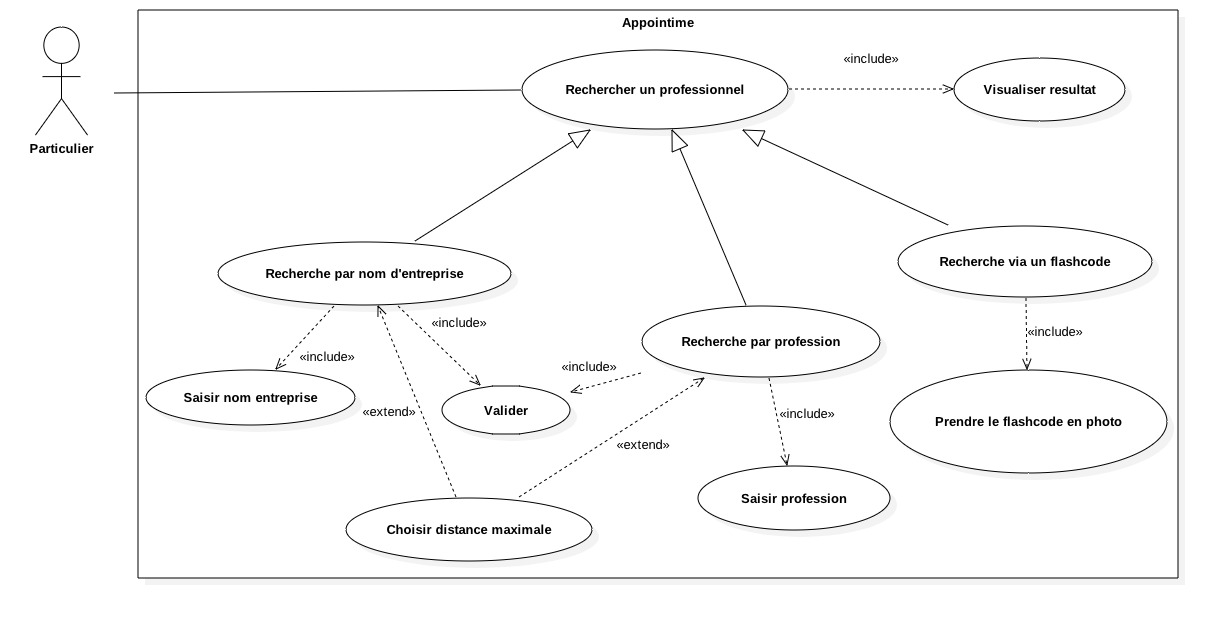
\includegraphics[scale=0.3]{ShematDiagrammes/useCaseRecherchePro.jpg}

\end{itemize}

\paragraph{Prise de rendez-vous chez un professionnel :}
\begin{itemize}

\item La séléction d'un
  professionnel de la liste doit permettre d'afficher le
  calendrier du professionnel en question.
\item Le client doit pouvoir selectionner une prestation parmis une liste
  proposée par le professionnel.
\item Après avoir selectionné une prestation, le système affiche le
  calendrier du professionnel avec les crénaux diponnibles et le
  client peut selectionner un crénau.
\item Une fois le crénau sélectionné, le client est redirigé vers
    une page recapitulative de sa prise de rendez-vous. Avec un bouton
    confirmer ou annuler.
\item Si le particulier confirme son choix, les details de ce rendez vous s'ajouteront a la liste des rendez 
vous en attente de confirmation dans la page "en attente de confirmation"
si la tâche n'est pas en confirmation automatique.
\item Les rendez vous confirmés par les deux parties (particulier et professionnel) seront listés dans la section "rendez vous a venir"
\item Lors de sa reservation, le client devrait pouvoir proceder au
  payment directement sur l'application si le rendez-vous est confirmé et si le professionnel accepte ce genre de payement.
\item Lors de sa réservation, le client devrait pouvoir ajouter des
  rappels de rendez-vous. Pour ajouter un rappel de rendez-vous, le
  client appuie sur \og ajouter un rappel \fg{} puis choisis quand le
  rappel va être fait (en nombre d'heure ou de jours avant le
  rendez-vous).

%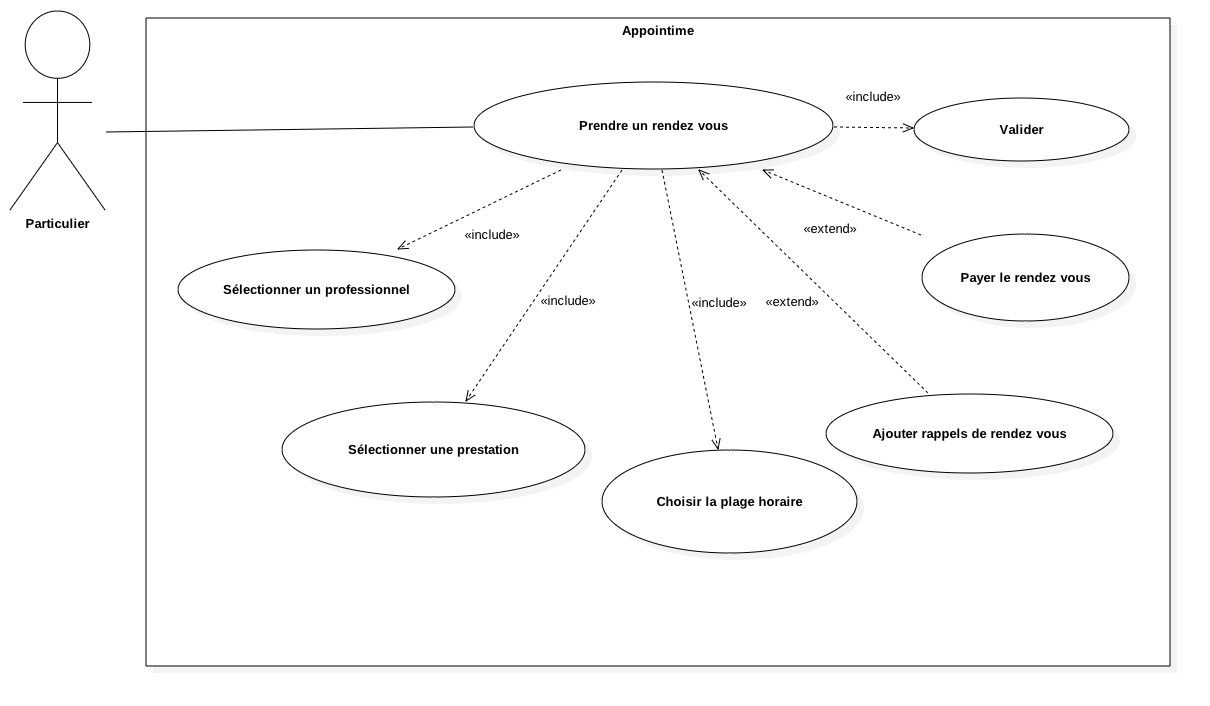
\includegraphics[scale=0.3]{ShematDiagrammes/useCasePriseRdv.jpg}


\end{itemize}


\paragraph{Paramétrage du calendrier côté profesionnel :}
\begin{itemize}
\item Un menu doit permettre au professionnel de créer une nouvelle
  prestation en appuyant sur un bouton \og Ajouter une prestation
  \fg{}.
\item Une liste déroulante doit permettre à l'utilisateur d'afficher
  les prestations déjà existantes. Chaque elements de la liste est
  accompagné des boutons \og selectionner \fg{}, \og modifier \fg{} et
  \og supprimer \fg{}.

\item Un formulaire doit permettre de créer une prestation. Ce
  formulaire doit contenir les champs textuels suivant \og Nom \fg{}, \og Description
 \fg{},  \og Durée \fg{}, \og Prix \fg{} et \og Validation automatique \fg{}.

%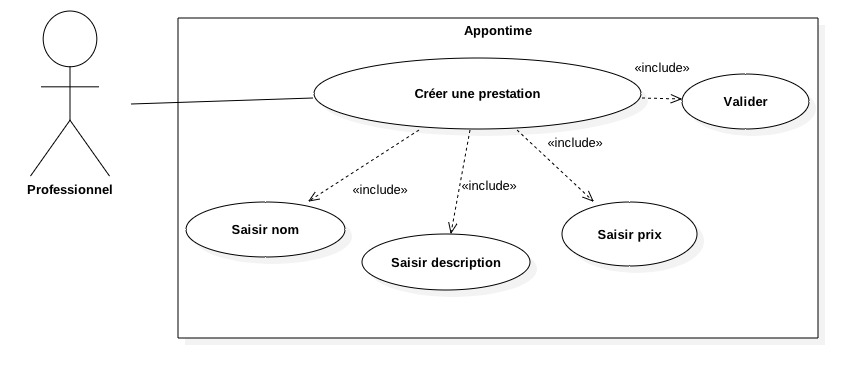
\includegraphics[scale=0.5]{ShematDiagrammes/useCaseCreerPrestation.jpg}

\item Un formulaire doit permettre d'éffectuer des modifications sur
  une prestation. Ce formulaire doit contenir un champ nom, un champ description, un champ
  durée, un champ prix et un champ validation automatique.
\item L'utilisateur doit pouvoir choisir si il souhaite une validation automatique ou manuelle des rendez-vous.
\item Un calendrier modifiable doit permettre à l'utilisateur de
  modifier ses diponibilitées en modifiant les jours et les horaires
  auquelles il peux effectuer ses prestations.
\item Le calendrier modifiable doit pemettre à l'utilisateur de
  visualiser et de gérer les rendez vous déjà pris. Sur un crénaux
  pris, il doit afficher les informations de l'utilisateur qui a pris
  le rendez-vous. Il doit aussi permettre au professionnel de valider
  ou non les rendez vous.
\end{itemize}

\paragraph{Acceptation de prise de rendez-vous}


Lorsqu'un rendez vous est pris par un particulier, le
  professionnel recoit une notification. Lorsque le professionnel
  appuie sur cette dernière, l'application souvre sur une page ou il
  est indiqué les informations de l'utilisateur et de la tâche a éffectuer.
\begin{itemize}
\item  Si la tache à effectuer est en validation manuelle: un bouton \og
  Accepter le rendez vous \fg{} et un bouton \og
  Refuser le rendez vous \fg{} seront présents dans la page décrite précedement.
\end{itemize}
\paragraph{Signalement des particulier}
\begin{itemize}
\item Si un rendez-vous à été pris par un particulier mais ce dernier
  n'y s'est pas rendu, le professionnel doit pouvoir
  signaler le particulier via un bouton \og signaler \fg{} situé
  à coté de chaque nom d'utilisateur son calendrier. Cette action retire un \og point de crédibilité \fg{} à l'utilisateur qui possède
  3 \og points de crédibilité \fg{}. Si l'utilisateur arrive à 0 point de crédibilité son compte est
  bloqué définitivement. L'utilisateur peut récuperer un point de crédibilité  en étant
  allé à 10 rendez-vous d'affilé.
\end{itemize}

\subsubsection{Interfaces avec les logiciels}
\paragraph{Gestion des notifications :}
L'application doit communiquer avec le système d'exploitation du
smarphone afin d'afficher, lorsque ceci est necessaire, des
notifications dans la barre de notifications du smartphone.

\subsubsection{Interface avec le materiel}
\paragraph{Identification par empreinte :}
L'application devrait communiquer avec le materiel si celui-ci dispose
d'un capteur d'empreinte digitale afin de pouvoir se connecter rapidement à
l'application grâce à ce mode d'identification.
\paragraph{Identification par reconaissance faciale :}
L'application devrait communiquer avec le materiel, si celui ci dispose
d'un technologie de reconnaissance faciale, afin de pouvoir se
connecter rapidement à l'application grâce à ce mode
d'indentification.
\paragraph{Recherche par flashcode}
\begin{itemize}
\item Pour pouvoir être recherché rapidement, chaque professionnel
  devrait posseder un flashcode unique.
\item Le particulier devrait pouvoir rechercher un professionnel par le
  biais de son appareil photo via un flashcode founi par le
  professionnel.
\end{itemize}

\subsubsection{Interface de comunication :}
L'application doit communiquer avec un serveur distant via internet
(Wifi ou réseau mobile) contenant la base de donnée de l'application et
les photos de profil des utilisateurs.


\subsection{Exigences fonctionnelles}
\paragraph{Pour la connexion : }

\begin{itemize}
\item Si l'email existe dans la base de données :
	le systeme doit vérifier si le mot de passe saisi
	correspond à l'email saisi.
		\begin{itemize}
		\item Si il correspond, le systeme doit autoriser la connexion et
			rediriger l'utilisateur à l'acceuil. Ce dernier aura accès à son
			profil ainsi qu'aux pages de reservation/gestion de calendrier
			si c'est un particulier/professionnel.
		\item Si il ne correspond pas, le systeme doit afficher une erreur
			et renvoyer sur la page de connexion
		\end{itemize}
\item Si il n'existe pas le systeme doit renvoyer une erreur
	et renvoyer sur la page de connexion.
\end{itemize}

%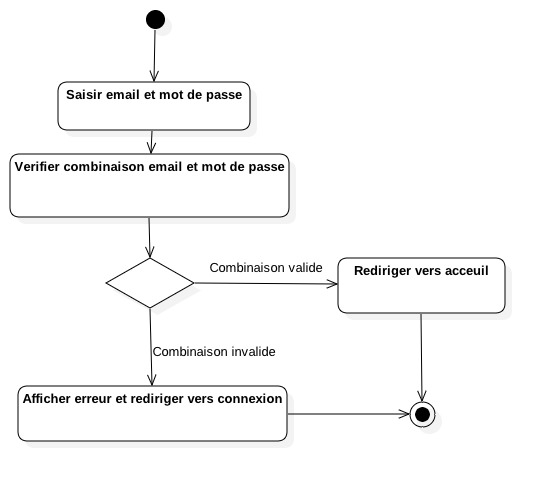
\includegraphics[scale=0.6]{ShematDiagrammes/activiteConnexion.jpg}

\paragraph{Pour l'inscription d'un utilisateur: }
\begin{itemize}
\item Le systeme doit verifier si les données saisies sont valides
	\begin{itemize}
	\item Si les données sont valides, le systeme doit verifier si le mail
		est deja existant.
		\begin{itemize}
		\item Si l'email n'existe pas encore dans la base de données le systeme
			doit les enregister,indiquer le bon deroulement de l'opération via un message temporaire et rediriger vers la page de connexion.
		\item Si l'email existe déja le systeme doit rediriger vers
			la page d'inscription et indiquer que le mail est déja utilisé
			via un message.
		\end{itemize}
	\end{itemize}
\item Si les données ne sont pas valides le systeme doit l'indiquer
	via un message détaillant les erreurs.
\end{itemize}

%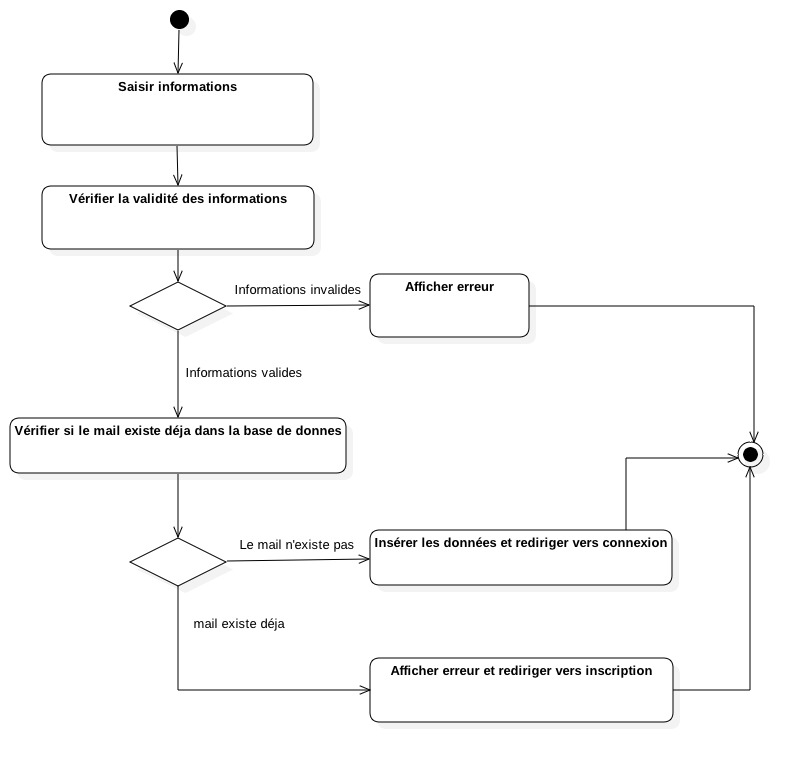
\includegraphics[scale=0.5]{ShematDiagrammes/activiteInscription.jpg}
\paragraph{Pour l'inscription d'une entreprise: }
\begin{itemize}
\item Le systeme doit verifier si les données saisies sont valides
	
		\begin{itemize}
		\item Si le numero de siret n'est pas encore utilisé, le système
			doit enregister les données,indiquer le bon deroulement de l'opération via un message temporaire et rediriger vers la page de gestion d'horaires d'ouverture.
		\item Si le numero de siret existe déja le systeme doit rediriger vers
			la page d'inscription d'entrprise et indiquer que le numéro de siret est déja utilisé
			via un message.
		\end{itemize}

\item Si les données ne sont pas valides le systeme doit l'indiquer
	via un message détaillant les erreurs.
\end{itemize}

\paragraph{Pour la gestion d'horaires d'ouverture d'une entreprise: }
\begin{itemize}
\item Le systeme doit verifier si les données saisies sont valides
	
		\begin{itemize}
		\item Si les données sont valides (heure d'ouverture superieure a l'heure de fermeture, l'heure ne correspond pas a la demie journée(matin/apres midi))le système
			doit enregister les données,indiquer le bon deroulement de l'opération via un message temporaire et rediriger vers la page de gestion d'horaires d'ouverture.
		\item Si les données ne sont pas valides le système doit rediriger vers
			la page de gestion d'horaires d'ouverture et indiquer les erreures
			via un message.
		\end{itemize}

\item Si les données ne sont pas valides le systeme doit l'indiquer
	via un message détaillant les erreurs.
\end{itemize}


\paragraph{Pour la gestion de compte : }
\begin{itemize}
\item Le systeme doit verifier si les données saisies sont valides
	\begin{itemize}
	\item Si les données sont valides:
		\begin{itemize}
		\item Le systeme remplace les données obsoletes par
                  les nouvelles données.
                \item Le système renvoie l'utilisateur vers la page d'accueil
                 après avoir indiqué via un message temporaire le bon déroulement de l'opération.
		\end{itemize}
		\item Si les données ne sont pas valides:
		\begin{itemize}
		\item Le systeme renvoie un message d'erreur decrivant
                  les erreurs.
                \item Le systeme renvoie l'utilisateur sur la page de
                  gestion de compte.
		\end{itemize}
	\end{itemize}
\end{itemize}

\paragraph{Format / validitée des données saisies}
\begin{itemize}
\item L'email  et la confirmation d'email sont valides si elles ce plient à l'expression régulière
  suivante :

[a-zA-Z0-9]+@[a-zA-Z0-9]+.[a-zA-Z]

\item Le mot de passe et la confirmation de mot de passe sont valides si ils contiennent entre 8 et 25
  caractères et si ils contiennent au moins une majuscule et une minuscule.

\item Le nom d'utilisateur est valide si il contient entre 3 et 10
  caractères.

\item Le numéro de téléphone est valide si il est composé d'exactement
  10 chiffres.

\item L'adresse est valide si elle est composée uniquement de lettres,
  de chiffres et de ponctuation.
\end{itemize}


\paragraph{Pour l'ajout de prestation}
\begin{itemize}
\item Le systeme doit verifier si les données saisies sont valides
	\begin{itemize}
	\item Si les données sont valides:
		\begin{itemize}
		\item le système doit insèrer les nouvelles données en base
                  de données.
                  \item le système doit rediriger l'utilisateur vers
                    la page de parametrage du calendrier.
		\end{itemize}
		\item Si les données ne sont pas valides:
		\begin{itemize}
		\item Le systeme renvoie un message d'erreur decrivant
                  les erreurs.
                \item Le système doit renvoyer l'utilisateur vers le
                  formulaire d'ajout de prestation.
		\end{itemize}
	\end{itemize}
\end{itemize}


\paragraph{Pour la reservation (coté particulier) :}
Avant la confirmation:
	\begin{itemize}
	\item Si le particulier confirme sa réservation, le système doit:
	\begin{itemize}
	\item Si la tâche n'est pas en confirmation automatique:
		\begin{itemize}
		\item Passer la plage horaire en "en attente de confirmation"
			(la plage horaire ne doit plus être reservable jusqu'a nouvel ordre).
		\item Ajouter la réservation (date, heure,lieu, type de reservation, durée, prix éstimé) dans la section "en attente de confirmation"
		\end{itemize}
		\end{itemize}
	\end{itemize}
Apres la confirmation le systeme doit :
		\begin{itemize}
		\item enregistrer les eventuels changements faits par le professionnel.
		\item déplacer la reservation de "en attente de confirmation" vers "rendez vous à venir"
		\end{itemize}


\paragraph{Pour la réservation (coté professionnel) :}
\begin{itemize}
\item Avant la confirmation le systeme doit :
	\begin{itemize}
	\item Ajouter la réservation dans la section "réservations à confirmer" du  proféssionnel.
    \item Notifier le professionnel d'une demande de réservation via mail, notification sur l'application et eventuellement sms (si le proféssionnel à confirmé l'option prévue à cet effet).
		La notification doit comprendre les informations sur cette reservation (date, heure,lieu, type de reservation, durée, prix éstimé)
		ainsi que des informations sur le particulier (profil, points de crédibilité, numero de téléphone)
	\end{itemize}
\item Pour la confirmation (si elle n'est pas automatique):
	\begin{itemize}
	\item Si le professionnel adapte la réservation au besoin du client:
		\begin{itemize}
		\item Le systeme doit enregistrer les données dans la base de données (modifications éventuelles du prix,durée).
		\end{itemize}
	\end{itemize}
	\begin{itemize}
    \item Le systeme doit placer la réservation dans la section "rendez vous a venir" et la supprimer de "réservations à confirmer"
	\end{itemize}
\end{itemize}

%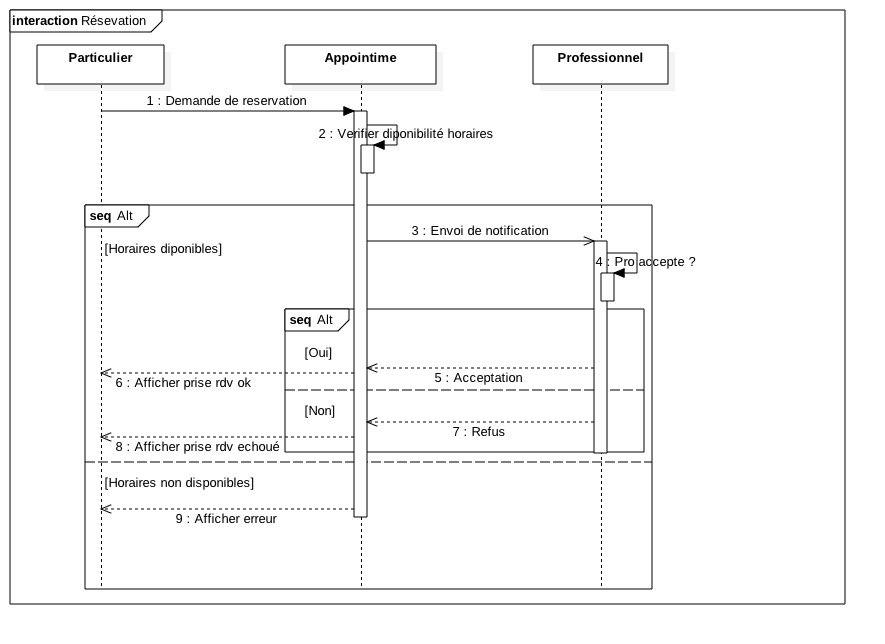
\includegraphics[scale=0.5]{ShematDiagrammes/sequenceReservation.jpg}





\paragraph{Pour la gestion du calendrier du professionnel :}
\begin{itemize}
\item Le systeme doit enregistrer les horaires du professionnel dans
  la base de données .
\item Le systeme doit enregistrer dans la base de données les taches
  prédefinie (prestations) que le professionnel souhaite ajouter.
\end{itemize}

\paragraph{Rappel de rendez-vous}
\begin{itemize}
\item Le systeme devrait enregistrer dans une base de données locale les
  rappels de rendez-vous définis par les utilisateurs.
\item Le systeme devrait afficher une notification et emmetre un son
  et/ou une vibration lorsque le l'heure du rappel de rendez vous est
  égale à l'heure du terminal.
\item Le system devrait ajouter une notification spéciale définit
  comme suit :
  \begin{itemize}
    \item Le systeme calcule le temps de voyage approximatif en minute
      noté X que le
      client mettra pour se rendre à son rendez-vous en voiture.
     \item Le systeme envoie alors un notification X+10 minutes avant
       le rendez-vous.
     \item Cette notification contient le nom du rendez-vous ainsi
       qu'une proposition d'itineraire GPS.
  \end{itemize}

\end{itemize}

\subsection{Exigences de performance}
\subsubsection{Exigences statiques}
\paragraph{Nombre d'utilisateurs simultané :}
L'application doit pouvoir supporter 50 utilisateurs/terminaux
simultanément.
\paragraph{Volume de données :}
Le système doit pouvoir dédier 20Mo par utilisateurs soit un total de
1000Mo pour au moins 50 utilisateurs.
\paragraph{Type des données :}
Les système doit pouvoir stocker des données de type entier, chaine de
caractères, booléen et une images 100x100 pixel par utilisateurs
(photo de profil).


\subsubsection{Exigences dymamiques}
\paragraph{Acces au serveur :}
Le système doit permettre un minimum de 50 requetes/reponses au serveur
par secondes.
\paragraph{Temps de latence :}
\begin{itemize}
\item En condition favorables (50 requetes/reponse par seconde) le
  système doit avoir un temps de latence maximal de 2 secondes dans
  90\% des cas.
\item En condition de surcharge du serveur (150 requete/reponse par
  seconde) le systèmes doit avoir un temps de latence maximal de 4
  secondes dans 75\% des cas.
\end{itemize}

\paragraph{Temps d'execution des tâches hors ligne :}
Le temps de calcul d'une tache simple sans acces au serveur (exemple : passage d'une vue a
une autre) doit êtres executé en 500 milisecondes maximum sur 65\% des
smartphones.

\paragraph{Temps pour une prise de rendez vous :}
Étant donné un utilisateur ayant utilisé l'application pendant 1
semaine, le temps moyen pour une prise de rendez-vous doit être dans
60\% des cas inférieur à 5 minutes.

\subsection{Exigences logiques relatives aux bases de données}
\subsubsection{Types d'informations utilisés}
\paragraph{Utilisateurs}
Pour les utilisateurs, nous devrons stocker
\begin{itemize}
\item Un identifiant (entier)
\item L'email (Chaine de caractères (entre 5 à 30 caractères))
\item Le nom d'utilisateur (Chaine de caractères (entre 3 et 10 caracteres))
\item Le mot de passe (Chaine de caractères (entre 8 et 25 caractères))
\item Le numero de téléphone (Chaine de caractères (exactement 10 caracteres)
\item L'adresse (Chaine de caractères (maximum 100 caractères))
\item Le fait que l'utilisateur soit professionnel ou non (booléen)
\end{itemize}

\paragraph{Entreprise}
Pour les entreprises, nous devrons stocker:
\begin{itemize}
\item Un identifiant (entier)
\item Une référence vers un utilisateur professionnel (id du professionnel(entier)) 
\item Une description du domaine d'activité (Chaine de caractères (maximum 100 caractères))
\item Une adresse (Chaine de caractères (maximum 100 caractères))
\item Une description générale(Chaine de caractères (maximum 100 caractères))
\item Un numero de siret(Chaine de caractères (14 caracteres))
\end{itemize}

\paragraph{Tâche}
Pour les tâches, nous devrons stocker
\begin{itemize}
\item Un identifiant (entier)
\item Une référence vers une entreprise (id de l'entreprise (entier))
\item Un titre (Chaine de caracteres (maximum 20 caractères))
\item Une description générale(Chaine de caractères (maximum 100 caractères))
\item Une durée d'execution (entier, en nombre de minutes)
\item Un prix (entier)
\item Une confirmation automatique (booléen)
\end{itemize}

\paragraph{Calendrier}
Pour les calendriers, nous devrons stocker
\begin{itemize}
\item Une référence vers une entreprise (id de l'entreprise (entier))
\item Un numéro de demi journée de la semaine (entier)
\item Une heure de début de service (date)
\item Une heure de fin de service (date)
\item Un indicateur d'ouverture (booléen)
\end{itemize}

\paragraph{Rendez-vous}
Pour les rendez-vous, nous devrons stocker
\begin{itemize}
\item Un identifiant (entier)
\item Une référence vers un utilisateur particulier (id du particulier (entier))
\item Une référence vers une tâche (id de la tache (entier))
\item L'heure de début (date)
\item L'heure de fin (date)
\end{itemize}

\subsubsection{Fréquence d'utilisation}


\section{Annexes}
poulet
\section{Index}


\end{document}
